\documentclass[a4paper,12pt,oneside]{book}

%%% Início do preâmbulo %%%

\usepackage[paper=a4paper,top=3cm,bottom=2.5cm,right=2.5cm,left=3cm]{geometry} % https://www.ctan.org/pkg/geometry
\usepackage[brazil]{babel} % https://www.ctan.org/pkg/babel
\usepackage[T1]{fontenc} % https://www.ctan.org/pkg/fontenc
\usepackage[utf8]{inputenc} % https://www.ctan.org/pkg/inputenc (usar no Linux)
%\usepackage[latin1]{inputenc} % (usar no MS Windows ou Mac OS X)
%\usepackage[applemac]{inputenc} % (usar no Macintosh)
\usepackage[12pt]{moresize} % https://ctan.org/pkg/moresize
\usepackage{textcomp} % https://www.ctan.org/pkg/textcomp
\usepackage{fixltx2e} % https://www.ctan.org/pkg/fixltx2e
%\usepackage{arev} % https://www.tug.org/FontCatalogue/arev/
%\usepackage{lmodern} % https://www.tug.org/FontCatalogue/latinmodernsans/
%\usepackage{avant} % https://www.ctan.org/pkg/psnfss
\usepackage{colortbl} % https://ctan.org/pkg/colortbl
\usepackage[dvipsnames,table]{xcolor} % https://www.ctan.org/pkg/xcolor
\usepackage[ddmmyyyy]{datetime} % https://www.ctan.org/pkg/datetime
\usepackage{indentfirst} % https://www.ctan.org/pkg/indentfirst
\usepackage{graphicx} % https://www.ctan.org/pkg/graphicx
\usepackage{wrapfig} % https://www.ctan.org/pkg/wrapfig
\usepackage{eso-pic} % https://www.ctan.org/pkg/eso-pic
\usepackage{sectsty} % https://www.ctan.org/pkg/sectsty
\usepackage{amsmath} % https://www.ctan.org/pkg/amsmath
\usepackage{amssymb} % https://www.ctan.org/pkg/amsfonts
\usepackage{stmaryrd} % https://www.ctan.org/pkg/stmaryrd
\usepackage[stable]{footmisc} % https://www.ctan.org/pkg/footmisc
\usepackage{tikz} % https://www.ctan.org/pkg/pgf
    \usetikzlibrary{matrix,shapes.misc,arrows,chains,trees}
\usepackage[all]{genealogytree} % https://www.ctan.org/pkg/genealogytree
\usepackage{pifont} % https://www.ctan.org/pkg/pifont
\usepackage{dirtytalk} % https://www.ctan.org/pkg/dirtytalk
\usepackage{paralist} % https://www.ctan.org/pkg/paralist
\usepackage[shortlabels]{enumitem} % https://www.ctan.org/pkg/enumitem
\usepackage{multicol} % https://www.ctan.org/pkg/multicol
\usepackage{multirow} % https://ctan.org/pkg/multirow
\usepackage{ragged2e} % https://www.ctan.org/pkg/ragged2e
\usepackage{vwcol} % https://www.ctan.org/pkg/vwcol
    \setlength{\columnsep}{0.5cm}
\usepackage{setspace} % https://www.ctan.org/pkg/setspace
\usepackage{verbatim} % https://www.ctan.org/pkg/verbatim
\usepackage{array} % https://www.ctan.org/pkg/array
\usepackage{lipsum} % https://www.ctan.org/pkg/lipsum
\usepackage[htt]{hyphenat} % https://ctan.org/pkg/hyphenat
\usepackage{tabularx} % https://www.ctan.org/pkg/tabularx

\usepackage[hidelinks]{hyperref} % https://www.ctan.org/pkg/hyperref
    \hypersetup{
    	colorlinks=false,
    	linkcolor=black,
		urlcolor=black,
		anchorcolor=black,
		citecolor=black,
		filecolor=black,
		linktoc=section,
		pdfstartview=,
		plainpages=false,
		pdfpagelabels=true,
		pdftitle={Tutorial básico de \LaTeX},
		pdfsubject={latex},
		pdfkeywords={tutorial;latex},
		pdfauthor={Daniel Madeira},
		pdfcreator={LaTeX no TeXstudio}, % software que editou o código LaTeX
		pdfproducer={TeX Live com pdfTeX}, % software que converteu para PDF
		pdfdisplaydoctitle=true
	}

\usepackage{fancyhdr} % https://www.ctan.org/pkg/fancyhdr
    \fancyhf{}
    \renewcommand{\headrulewidth}{0pt}
    \cfoot{\thepage}
    \pagestyle{fancy}

\renewcommand{\familydefault}{\sfdefault} % estabelece o uso da fonte sem serifa como padrão.
\renewcommand{\familydefault}{\rmdefault} % estabelece o uso da fonte roman como padrão.

\newcommand*{\justifytt}{%
	\fontdimen2\font=0.4em% interword space
	\fontdimen3\font=0.2em% interword stretch
	\fontdimen4\font=0.1em% interword shrink
	\fontdimen7\font=0.1em% extra space
	\hyphenchar\font=`\-% allowing hyphenation
}

\newenvironment{folharosto}[1]
	{\begin{center}
		\vspace*{\fill}
		{\LARGE #1}\par
		\vspace{2cm}
    }
    {
		\vspace*{\fill}
		\thispagestyle{empty}
		\renewcommand{\thepage}{rosto}
    \end{center}
    }

\title{Tutorial básico de \LaTeX} % define o título do documento.
\author{Daniel Madeira} % define o autor do documento.
\date{\today} % define a data do documento.

%%% Fim do preâmbulo %%%

\begin{document}

\begin{titlepage}
    \AddToShipoutPictureBG*{
\includegraphics[width=\paperwidth,height=\paperheight]{clouds.jpg}}
    \maketitle
    \thispagestyle{fancy}
    \renewcommand{\thepage}{capa}
\end{titlepage}

\pagecolor{gray!5!yellow!5}

\begin{folharosto}{Tutorial básico de \LaTeX}
	Um tutorial prático no formato .tex.
\end{folharosto}

\frontmatter

\tableofcontents

\mainmatter

%\counterwithout{section}{chapter} % conta as seções sem incluir o número do capítulo

\setlength{\parskip}{1em}

\chapter*{Prefácio}
\addcontentsline{toc}{chapter}{Prefácio}

O \LaTeX\ é um sistema de preparação de documento com alta qualidade para composição tipográfica. É utilizado para criar documentos dos mais variados tipos de publicação, como artigos, teses, dissertações, livros, cartas, relatórios ou qualquer outro tipo de documento. Possui um alto grau de exatidão e precisão na diagramação do conteúdo do documento e alta qualidade na formatação automática do documento. O \LaTeX\ é uma ampliação do original sistema de tipografia \TeX. Tornou-se um padrão para produção de documentos científicos.

O sistema \LaTeX\ possui código aberto e é gratuito. Está disponível para qualquer sistema operacional, produzindo o mesmo resultado em qualquer sistema. Cria arquivos pequenos e com resultados de alta qualidade. É capaz de exportar o documento para os formatos Post Script e PDF.

Este tutorial tem o propósito de mostrar o mínimo, o básico, para se conseguir produzir um documento, de uma forma prática. O próprio arquivo .tex deste tutorial é um exemplo básico da linguagem em \LaTeX.

\chapter*{Linguagem \LaTeX}
\addcontentsline{toc}{chapter}{Linguagem \LaTeX}

\section*{Arquivo}
\addcontentsline{toc}{section}{Arquivo}

O arquivo do código-fonte em \LaTeX\ deve conter apenas bytes que representem caracteres, sem nenhuma informação adicional. Trata-se do denominado arquivo de texto plano (txt). Este arquivo recebe a extensão .tex. A codificação recomendada para este arquivo é a codificação UTF-8 ou Latin1, dependendo do sistema operacional que está processando o \LaTeX.

Pode-se utilizar qualquer editor de texto puro para produzir o arquivo .tex, entretanto, é recomendável utilizar um editor \LaTeX\ para obter uma melhor produtividade. Basicamente, precisa estar instalado no computador: uma distribuição \TeX, por exemplo TeX Live ou MikTex; e um editor \LaTeX, por exemplo TeXstudio, Texmaker ou TeXworks.

Atente-se: Editar um documento em \LaTeX\ não será WYSIWYG ("What You See Is What You Get"). Será literalmente editar o código-fonte do documento, inserindo os comandos de formatação do texto.

\section*{Estrutura do código}
\addcontentsline{toc}{section}{Estrutura do código}

\subsection*{Partes}
\addcontentsline{toc}{subsection}{Partes}

\begin{multicols}{2}
A estrutura global do código-fonte\\ em \LaTeX\ é basicamente:
\columnbreak
\begin{verbatim}
	\documentclass{...}
	\begin{document}
	...
	\end{document}
\end{verbatim}
\end{multicols}

A área entre \texttt{\textbackslash documentclass\{...\}} e \texttt{\textbackslash begin\{document\}} é denominada preâmbulo. Neste preâmbulo ficam os comando que afetam todo o documento. Como as chamadas do uso de pacotes, definições de parâmetros de comandos, criação de novos comandos, recriação de comandos existentes etc.

A área entre \texttt{\textbackslash begin\{document\}} e \texttt{\textbackslash end\{document\}}, após o preâmbulo, forma o bloco principal, o ambiente do documento, é onde fica todo o conteúdo do documento.

\subsection*{Ambiente}
\addcontentsline{toc}{subsection}{Ambiente}

Na linguagem \LaTeX, um bloco é definido entre os comandos \texttt{\textbackslash begin\{\}} e \texttt{\textbackslash end\{\}}. Estes comandos formam o bloco de ambiente. Os comandos inseridos dentro deste ambiente tem seu efeito restrito ao interior do bloco.

\subsection*{Caracteres especiais}
\addcontentsline{toc}{subsection}{Caracteres especiais}

Quase tudo pode ser digitado livremente no documento, que fará parte da impressão final, salvo alguns caracteres que são considerados especiais. Estes caracteres simbólicos são reservados pela linguagem \LaTeX\ porque são para introduzir comandos e possuem um significado especial: \texttt{\# \$ \% \textasciicircum\ \& \_ \{ \} \textasciitilde\ \textbackslash}

Saiba a função de cada um deles:

\begin{small}
\begin{tabular}{lll}
	Caractere & Função & Como imprimir no PS/PDF\\
	\hline
	\#    & parâmetro de macro  & \texttt{\textbackslash\#}\\
	\$    & modo matemático & \texttt{\textbackslash \$}\\
	\%    & linha de comentário & \texttt{\textbackslash \%}\\
	\^{}  & sobrescrito (no modo matemático) & \texttt{\textbackslash\^{}\{\}} or \texttt{\textbackslash textasciicircum}\\
	\&    & separador de colunas & \texttt{\textbackslash \&}\\
	\_    & subscrito (no modo matemático) & \texttt{\textbackslash\_}\\
	\{ \} & bloco de processamento & \texttt{\textbackslash\{ \textbackslash\}}\\
	\~{}  & espaço inquebrável & \texttt{\textbackslash textasciitilde} or \texttt{\textbackslash\~{}\{\}}\\
	\textbackslash & início de comando & \texttt{\textbackslash textbackslash} or \texttt{\textbackslash}\\
\end{tabular}
\end{small}

Para usar (imprimir) algum destes caracteres no seu texto, digite com o caractere \texttt{\textbackslash} ou use o comando de impressão.

\subsection*{Comentário}
\addcontentsline{toc}{subsection}{Comentário}

\begin{multicols}{2}
É possível inserir comentários no código-fonte do documento em \LaTeX. Os comentários de uma linha ficam após o caractere \%. Os comentários com mais de uma linha ficam em um bloco de ambiente \texttt{\{comment\}}:
\columnbreak
\begin{verbatim}
\% comentário de uma linha.
\begin{comment}
    Bloco de comentário
    com mais de uma linha.
\end{comment}
\end{verbatim}
\end{multicols}

\section*{Pacotes}
\addcontentsline{toc}{section}{Pacotes}

O \LaTeX\ inclui alguns comandos básicos porém existem muitos outros comandos úteis que são implementados com o uso de pacotes no código-fonte. Alguns pacotes podem receber parâmetros:
\begin{verbatim}
	\usepackage[ddmmyyyy]{datetime}
\end{verbatim}

\section*{Comandos}
\addcontentsline{toc}{section}{Comandos}

O \LaTeX\ é uma linguagem movida por comandos (ou macros) no entorno do texto. Os comando são discriminados pelo caractere \textbackslash, escrito em uma sintaxe como \texttt{\textbackslash comando}.

O primeiro comando no código-fonte em \LaTeX\ é o comando \texttt{\textbackslash documentclass}. Nele se define a classe do documento (ex. article, report, book, letter, slides, ltnews, beamer ou memoir) e os parâmetros para tamanho do papel, tamanho da fonte, lados de impressão etc.:
\begin{verbatim}
	\documentclass[a4paper,12pt,oneside]{book}
\end{verbatim}


\subsection*{Definição e redefinição}
\addcontentsline{toc}{subsection}{Definição e redefinição}

A linguagem \LaTeX\ permite criar novos comandos, através do comando \texttt{\textbackslash newcommand}. O novo comando recebe um nome e uma definição. Isto possibilita, por exemplo, um modo de criar uma variável:
\begin{footnotesize}
\begin{verbatim}
\newcommand{\nomeVariavel}{valor}
\newcommand{\agua}{H$_2$O}
\end{verbatim}
\end{footnotesize}

Os comandos existentes podem ser redefinidos com o comando \texttt{\textbackslash renewcommand}, por exemplo:
\begin{footnotesize}
\begin{verbatim}
\renewcommand*\contentsname{Sumário} % refaz o termo para TOC.
\renewcommand*{\thepage}{capa} % string capa no número da página
\end{verbatim}
\end{footnotesize}

Criar e recriar comandos no \LaTeX\ vai muito além, não limitando-se somente a um valor para a definição. É possível criar combinações de comandos para compôr a definição do novo comando, inclusive a possibilidade de inserção de argumentos. A sintaxe básica é:
\begin{verbatim}
\newcommand{\nome}[n]{definição}
\end{verbatim}

Sendo n indicando o número de argumentos para uso pelo novo comando. Por exemplo, este novo comando que define um novo modo de inserir os capítulos:
\begin{footnotesize}
\begin{verbatim}
\newcommand{\meucapitulo}[2]{
	\setcounter{chapter}{#1}
	\setcounter{section}{0}
	\chapter*{#2}
	\addcontentsline{toc}{chapter}{#2}
}
\end{verbatim}
\end{footnotesize}

Ou este, por exemplo, que cria um comando para justificar um texto com fonte teletipo (texttt):
\begin{footnotesize}
\begin{verbatim}
\newcommand*{\justifytt}{%
	\fontdimen2\font=0.4em%
	\fontdimen3\font=0.2em%
	\fontdimen4\font=0.1em%
	\fontdimen7\font=0.1em%
	\hyphenchar\font=`\-%
}
\end{verbatim}
\end{footnotesize}

Duas observações:

Primeiro, perceba o caractere de asterisco em \texttt{\textbackslash newcommand} e \texttt{\textbackslash renewcommand}. Na origem da linguagem \TeX\ os comandos não podiam ter um \texttt{\textbackslash par} na definição. A linguagem \LaTeX\ controla a possibilidade disso com a ausência ou presença do asterisco na chamada do comando. Com o asterisco, o comando não aceita parágrafos dentro da definição do comando.

Segundo, perceba o caractere \% no fim das linhas. Alguns comandos que lidam precisamente com espaços entre os caracteres, se comportam melhor quando é inserido o \% no final da linha.

\subsection*{Uso}
\addcontentsline{toc}{subsection}{Uso}

A sintaxe geral de uso de um comando é:
\begin{footnotesize}
\begin{verbatim}
\comando[argumento opcional]{argumento compulsório}
\end{verbatim}
ou
\begin{verbatim}
\comando{argumento compulsório}[argumento opcional]
\end{verbatim}
\end{footnotesize}

O nome do comando é sensível a letras maiúsculas e minúsculas e compõe somente de caracteres alfa-numéricos. Os argumentos podem ser mais de um, se houver.

\subsection*{Unidades de medida}
\addcontentsline{toc}{subsection}{Unidades de medida}

As unidades de medidas aceitas nos comandos do LaTeX são:

\begin{tabular}{ll}
pt & pontos\\
mm & milímetros\\
cm & centímetros\\
in & polegadas\\
ex & altura de um x minúsculo na fonte corrente\\
em & largura de um M maiúsculo na fonte corrente\\
mu & unidade matemática igual à 1/18em\\
\end{tabular}

Muitos comandos aceitam valores negativos, por exemplo \texttt{\textbackslash hspace\{-1.5em\}}.

\subsection*{Cores}
\addcontentsline{toc}{subsection}{Cores}

Com o uso do pacote xcolor é possível definir cores para o texto, fundo do texto, fundo da página, linhas e colunas de tabelas, gráficos etc. Pode-se usar as cores pré-definidas ou definir novas cores usando valores em RGB, Hex ou CMYK. Inicialmente, com o uso do pacote xcolor, existem algumas cores pré-definidas, que são:

\texttt{\small\justifytt\color{blue} black, blue, brown, cyan, darkgray, gray, green, lightgray, lime, magenta, olive, orange, pink, purple, red, teal, violet, white, yellow.}

Se o pacote foi carregado com a opção \texttt{[dvipsnames]}, então um total de 68 cores estarão pré-definidas:

\texttt{\small\justifytt\color{OliveGreen} Apricot, Aquamarine, Bittersweet, Black, Blue, BlueGreen, BlueViolet, BrickRed, Brown, BurntOrange, CadetBlue, CarnationPink, Cerulean, CornflowerBlue, Cyan, Dandelion, DarkOrchid, Emerald, ForestGreen, Fuchsia, Goldenrod, Gray, Green, GreenYellow, JungleGreen, Lavender,
LimeGreen, Magenta, Mahogany, Maroon, Melon, MidnightBlue, Mulberry, NavyBlue, OliveGreen, Orange, OrangeRed, Orchid, Peach, Periwinkle, PineGreen, Plum, ProcessBlue, Purple, RawSienna, Red, RedOrange, RedViolet, Rhodamine, RoyalBlue, RoyalPurple, RubineRed, Salmon, SeaGreen, Sepia, SkyBlue, SpringGreen, Tan, TealBlue, Thistle, Turquoise, Violet, VioletRed, White, WildStrawberry, Yellow, YellowGreen, YellowOrange.}

Para definir novas cores, insira os comandos no preâmbulo, seguindo estes exemplos:
\begin{footnotesize}
\begin{verbatim}
\definecolor{cinza}{gray}{0.95}
\definecolor{laranja}{RGB}{255,127,0}
\definecolor{laranja}{HTML}{FF7F00}
\definecolor{laranja}{cmyk}{0,0.5,1,0}
\end{verbatim}
\end{footnotesize}

Ou ainda, crie uma mistura de cores, por exemplo:
\begin{verbatim}
\colorlet{azurelo}{blue!50!yellow}
\end{verbatim}

Para cada lugar de uso das cores, um comando específico será utilizado. Por exemplo, o texto é colorizado com \texttt{\textbackslash textcolor\{\textit{cor}\}}, uma linha de tabela com \texttt{\textbackslash rowcolor\{\textit{cor}\}} e por aí vai. Em todos estes comandos, a cor é referenciada pelo seu nome no argumento do comando.

A cor pode ser implementada integralmente, com 100\% de sua intensidade, ou reduzida em sua intensidade ou até misturada com outras cores. Para a redução de intensidade usa-se a sintaxe com seu nome + exclamação + valor, por exemplo: \texttt{blue!60}. A mistura de cores funciona acrescentando mais uma exclamação e o nome da segunda cor, que também pode ter sua intensidade reduzida, por exemplo: \texttt{blue!60!yellow}. 

Um exemplo de comando completo:

\texttt{\textcolor{red!50!violet!90}{ \textbackslash textcolor\{red!50!violet!90\}\{seu texto\} }}

\newgeometry{margin=4.5cm,nohead} % nova disposição desta página em diante

\chapter*{Formatação da página}
\addcontentsline{toc}{chapter}{Formatação da página}

\section*{Margens}
\addcontentsline{toc}{section}{Margens}

O pacote geometry proporciona um meio de configurar a disposição da página. Por exemplo, esta página está com a margem de 4,5cm e sem o espaço do cabeçalho (veja o código-fonte).

Basicamente usa-se dois comandos, um para definir e outro para restaurar o que foi definido no preâmbulo:
\begin{verbatim}
\newgeometry{top=1.5cm,bottom=1.5cm,right=1cm,left=1cm}

\restoregeometry
\end{verbatim}

Ambos os comandos implicam em uma quebra de página, para fazer valer a alteração na dimensão.

\restoregeometry % restaura a geometria definida no carregamento do pacote. Irá ter uma quebra de página aqui.

\section*{Quebras de página}
\addcontentsline{toc}{section}{Quebras de página}

Além dos comandos de geometria de página, há outros específicos para impor uma quebra na página. Basicamente são os comandos:
\begin{verbatim}
\pagebreak
\newpage
\clearpage
\end{verbatim}

O comando \texttt{\textbackslash pagebreak} faz com que os parágrafos se desloquem para preencher toda página, para não deixar espaço vazio no fim. Diferentemente, o comando \texttt{\textbackslash newpage} não estica os espaços entre os parágrafos, deixando um grande espaço vazio no fim da página. O comando \texttt{\textbackslash clearpage} é similar ao \texttt{\textbackslash newpage}, apenas agindo também nas figuras (mas ainda não testei).

\subsection*{Mesma página}
\addcontentsline{toc}{subsection}{Mesma página}

Caso tenha um conteúdo que queira manter-se em uma mesma página, sem quebra pelo meio, use o ambiente \texttt{\{samepage\}}.
\begin{verbatim}
\begin{samepage}
	...
\end{samepage}
\end{verbatim}

\section*{Espaço vazio}
\addcontentsline{toc}{section}{Espaço vazio}

É possível adicionar espaços vazios entre os conteúdos na página. Basicamente existe os comandos para espaço horizontal, que empurra o próximo conteúdo horizontalmente, e para espaço vertical, que empurra o próximo conteúdo verticalmente (valores negativos realizam o inverso, contraem o espaço). Os comandos são:
\begin{verbatim}
\hspace{medida}
\vspace{medida}
\end{verbatim}

Exemplos:
\begin{verbatim}
\hspace{1.5em}
\vspace{4cm}
\end{verbatim}

Quando for lidar com letras e palavras, use a unidade de medida em, pois esta unidade é proporcional ao tamanho e família da fonte do texto.

Uma interessante utilidade, caso queira posicionar os primeiros parágrafos no topo da página e os últimos parágrafos no fim da página, use um destes dois comandos equivalentes para esticar o espaço vazio entre eles:
\begin{verbatim}
\vspace{\fill}

\vfill
\end{verbatim}

\vspace{3cm} % insere um espaço vazio

Por exemplo, este parágrafo foi para baixo com \texttt{\textbackslash vspace\{3cm\}}. Obs.: Usando \texttt{\textbackslash vspace*} (com asterisco) o \LaTeX\ não remove o espaço vertical do fim da página (a documentação oficial também é confusa nesta explicação).

\section*{Estilo}
\addcontentsline{toc}{section}{Estilo}

Para limpar o estilo aplicado, na página atual ou nas próximas páginas, use um destes comandos com o estilo desejado:
\begin{verbatim}
\thispagestyle{empty}

\pagestyle{plain}
\end{verbatim}

O estilo empty limpa tanto o cabeçalho quanto o rodapé. No estilo plain, que é o padrão, o cabeçalho fica vazio e o rodapé contém o número da página no centro.

\section*{Colorindo}
\addcontentsline{toc}{section}{Colorindo}

Uma ou mais páginas podem ser coloridas com o comando \texttt{\textbackslash pagecolor\{\}}. Este comando terá efeito da página atual em diante. Por exemplo:
\begin{verbatim}
\pagecolor{gray!10!yellow!10}
\end{verbatim}

Para cancelar a definição da cor na página atual em diante, use o comando:
\begin{verbatim}
\nopagecolor
\end{verbatim}

\chapter*{Seções no documento}
\addcontentsline{toc}{chapter}{Seções no documento}

\section*{Níveis de seção}
\addcontentsline{toc}{section}{Níveis de seção}

O documento em \LaTeX\ pode ser seccionado em até 7 níveis, dependendo da classe declarada. As divisões de conteúdo no documento podem ser:

\begin{tabular}{lrcl}
	\textbf{Divisão} & \textbf{Nível} & & \textbf{Comando}\\
	\hline
	parte         & -1 & & \texttt{\textbackslash part\{\textit{nome}\}}\\
	capítulo      & 0  & & \texttt{\textbackslash chapter\{\textit{nome}\}}\\
	seção         & 1  & & \texttt{\textbackslash section\{\textit{nome}\}}\\
	subseção      & 2  & & \texttt{\textbackslash subsection\{\textit{nome}\}}\\
	subsubseção   & 3  & & \texttt{\textbackslash subsubsection\{\textit{nome}\}}\\
	parágrafo     & 4  & & \texttt{\textbackslash paragraph\{\textit{nome}\}}\\
	subparágrafo  & 5  & & \texttt{\textbackslash subparagraph\{\textit{nome}\}}\\
	\hline
\end{tabular}

Basta usar o comando do nível desejado e o que vier depois será desta divisão. Não há comando de encerramento, o próximo comando da próxima divisão é que indica a mudança. Exemplo:
\begin{small}
\begin{verbatim}
\begin{documenx}
\tableofcontents
\chapter{Introdução}
...
\chapter{Materiais}
\section{Líquidos}
...
\section{Sólidos}
\subsection{Descartáveis}
...
\subsection{Não-descartáveis}
...
\chapter{Conclusão}
...
\end{documenx}
\end{verbatim}
\end{small}

Os comandos destes níveis podem ser escritos na sintaxe sem o caractere *, desta forma, são numerados, prefixados com o número e adicionados automaticamente no sumário do documento. Com a utilização do *, logo após o nome do comando, nada disso acontece, então, para incluí-los no sumário adicione mais um comando. Exemplos para algumas divisões:
\begin{small}
\begin{verbatim}
\chapter*{Nome do Capítulo}
\addcontentsline{toc}{chapter}{Nome do Capítulo}

\section*{Nome da Seção}
\addcontentsline{toc}{section}{Nome da Seção}

\subsection*{Nome da Subseção}
\addcontentsline{toc}{subsection}{Nome da Subseção}
\end{verbatim}
\end{small}

\section*{Livro}
\addcontentsline{toc}{section}{Livro}

Em documentos da classe book, opcionalmente pode-se seccionar o conteúdo em quatro partes: frontal, principal, apêndice e traseira.

Tradicionalmente, a parte frontal contém a página do título, folha de rosto, resumo, sumário, prefácio, lista de figuras e lista de tabelas. A parte principal contém o conteúdo propriamente dito. Logo após existe o apêndice e a parte traseira contém o glossário, notas, bibliografia e índice.

São quatro comandos que definem estas partes:
\begin{verbatim}
\frontmatter
\mainmatter
\appendix
\backmatter
\end{verbatim}

A parte em \texttt{\textbackslash frontmatter} terá a numeração romana nas páginas e não terá os capítulos numerados. A parte em \texttt{\textbackslash mainmatter} terá o comportamento padrão do documento e a sequencia numérica das páginas é reiniciada. A parte \texttt{\textbackslash appendix} reinicia a numeração de capítulos com letras e continua seguindo a numeração das páginas principais. A parte \texttt{\textbackslash backmatter} continua seguindo a numeração das páginas principais mas volta a desativar a numeração dos capítulos.

\appendix resets chapter numbering, uses letters for chapter numbers and doesn't fiddle with page numbering;

\chapter*{Formatação de texto}
\addcontentsline{toc}{chapter}{Formatação de texto}

\section*{Parágrafo}
\addcontentsline{toc}{section}{Parágrafo}

\subsection*{Quebras de parágrafo e linha}
\addcontentsline{toc}{subsection}{Quebras de parágrafo e linha}

Isto é um texto em um parágrafo. O alinhamento justificado é aplicado por padrão. A linha se estica horizontalmente para ocupar todo o espaço entre as margens.

Para iniciar um novo parágrafo basta pular uma linha no código-fonte do \LaTeX.

Ou usar o comando \texttt{\textbackslash par} no final da linha; \par Para quebrá-la em um novo parágrafo.

Isto é um texto em uma linha, \newline o comando \texttt{\textbackslash newline} ou \texttt{\textbackslash\textbackslash} (duas barras invertidas) faz uma quebra de linha, sem criar um novo parágrafo.

\subsection*{Espaçamento entre parágrafos}
\addcontentsline{toc}{subsection}{Espaçamento entre parágrafos}

Os parágrafos, por padrão, não possuem um espaçamento entre eles diferente da separação simples entre linhas. Use esta combinação de comandos para definir um espaçamento dos próximos parágrafos:
\begin{verbatim}
\setlength{\parskip}{1em}
\end{verbatim}

\setlength{\parskip}{1em} % define um espaçamento entre os parágrafos (padrão é 0).

Perceba que este parágrafo já possui 1em de distância do parágrafo anterior e também do próximo parágrafo abaixo.

De agora em diante, todos os parágrafos terão este espaçamento entre eles.

\subsection*{Espaçamento entre linhas}
\addcontentsline{toc}{subsection}{Espaçamento entre linhas}

Por padrão, ocorre o espaçamento simples entre as linhas. Alguns comandos modificam isso, do pacote setspace:

\begin{verbatim}
\onehalfspacing
\doublespacing
\singlespacing

\renewcommand{\baselinestretch}{0.80}\normalsize
\renewcommand{\baselinestretch}{1}\normalsize
\end{verbatim}

Seguem os quatro exemplos para 0,80, simples(1), 1,5 e duplo:

\renewcommand{\baselinestretch}{0.80}\normalsize % outra forma de definir o espaçamento.
\lipsum[11]

\singlespacing % espaçamento simples entre as linhas (padrão).
\lipsum[11]

\onehalfspacing % espaçamento de 1,5 entre as linhas
\lipsum[11]

\doublespacing % espaçamento duplo entre as linhas.
\lipsum[11]

\renewcommand{\baselinestretch}{1}\normalsize % valor 1 é o simples.

\newpage

\subsection*{Espaçamento entre palavras}
\addcontentsline{toc}{subsection}{Espaçamento entre palavras}

Além do espaço comum (proveniente da tecla de espaço) entre as palavras, existem alguns comandos que alteram o espaço para mais ou menos.

\begin{tabular}{ll}
\textbf{Comando} &	\textbf{Descrição}
\\
\hline
\texttt{\textbackslash quad} &	espaço igual ao tamanho da fonte corrente (18 mu)
\\
\texttt{\textbackslash ,} &	3/18 de \textbackslash quad (3 mu)
\\
\texttt{\textbackslash :} &	4/18 de \textbackslash quad (4 mu)
\\
\texttt{\textbackslash ;} &	5/18 de \textbackslash quad (5 mu)
\\
\texttt{\textbackslash !} &	-3/18 de \textbackslash quad (-3 mu)
\\
\texttt{\textbackslash } {\footnotesize (espaço após a barra)} &	equivalente ao espaço no texto normal
\\
\texttt{\textbackslash qquad} &	dobro de \textbackslash quad (36 mu) 
\end{tabular}

Obs.: É comum em alguns comandos em linha, se houver uma continuação de texto após, mesmo que se tenha digitado um espaço, o conteúdo é impresso sem o espaço. Para resolver isto, inclua uma barra invertida antes deste espaço.

\subsection*{Indentação}
\addcontentsline{toc}{subsection}{Indentação}

Os parágrafos costumam indentar-se automaticamente. Mas, em uma instalação padrão, o primeiro não se indenta. Se não tivesse instalado o pacote indentfirst, este primeiro parágrafo não estaria indentado.

Para definir um tamanho de indentação, usa-se, antes dos parágrafos:
\begin{verbatim}
\setlength{\parindent}{3em}
\end{verbatim}

\setlength{\parindent}{3em} % define a largura da indentação (1.5em é o padrão).
Por exemplo, este parágrafo está com 3em de tamanho na indentação.

\noindent
Já este parágrafo não está indentado, pois usou o comando \texttt{\textbackslash noindent}.

\setlength{\parindent}{1.5em}
Voltando à indentação normal, com \texttt{\textbackslash setlength\{\textbackslash parindent\}\{1.5em\}}.

\indent Força uma indentação, caso não ocorra, mas só se parindent não estiver em zero.

\subsection*{Alinhamento}
\addcontentsline{toc}{subsection}{Alinhamento}

Outras formas de alinhamento podem ser aplicadas com o comando \texttt{\textbackslash begin ... \textbackslash end}. Como já visto, estes comandos criam um ambiente de formatação de bloco de texto. Existem outros três alinhamentos além do padrão justificado:

\newpage
\begin{center}
	Conteúdo centralizado na página,\\ definido com \texttt{\textbackslash begin\{center\} ...  \textbackslash end\{center\}}. 
\end{center}

\begin{flushleft}
	Conteúdo alinhado à esquerda,\\ definido com \texttt{\textbackslash begin\{flushleft\} ... \textbackslash end\{flushleft\}}.
\end{flushleft}

\begin{flushright}
	Conteúdo alinhado à direita,\\ definido com \texttt{\textbackslash begin\{flushright\} ... \textbackslash end\{flushright\}}.
\end{flushright}

\section*{Fontes}
\addcontentsline{toc}{section}{Fontes}

\subsection*{Tamanho}
\addcontentsline{toc}{subsection}{Tamanho}

Existem alguns tamanhos para os caracteres da fonte (e incrementado pelo pacote moresize), a partir do normal definido entre 10pt, 11pt ou 12pt, os quais são ativados por comandos com sintaxe inline ou para bloco de ambiente:

\begin{tabular}{lr}
	\tiny{Texto miúdo} & \texttt{\textbackslash tiny\{\}}\\
	\ssmall{Texto ppequeno} & \texttt{\textbackslash ssmall\{\}}\\
	\scriptsize{Texto script} & \texttt{\textbackslash scriptsize\{\}}\\
	\footnotesize{Texto rodapé} & \texttt{\textbackslash footnotesize\{\}}\\
	\small{Texto pequeno} & \texttt{\textbackslash small\{\}}\\
	\normalsize{Texto normal} & \texttt{\textbackslash normalsize\{\}}\\
	\large{Texto largo} & \texttt{\textbackslash large\{\}}\\
	\Large{Texto Largo} & \texttt{\textbackslash Large\{\}}\\
	\LARGE{Texto LARGO} & \texttt{\textbackslash LARGE\{\}}\\
	\huge{Texto imenso} & \texttt{\textbackslash huge\{\}}\\
	\Huge{Texto Imenso} & \texttt{\textbackslash Huge\{\}}\\
	\HUGE{Texto IMENSO} & \texttt{\textbackslash HUGE\{\}}\\
\end{tabular}

Outra forma de sintaxe inline é: \texttt{\{\textbackslash small ... \}}.

\begin{normalsize}
Uma outra maneira, de definir o tamanho do texto, é em um ambiente com bloco de parágrafo. Exemplo:

\texttt{\textbackslash begin\{large\}\\
\indent...\\
\indent\textbackslash end\{large\}}.
\end{normalsize}

\subsection*{Estilo}
\addcontentsline{toc}{subsection}{Estilo}

Os diversos estilos para os caracteres são:

\begin{tabular}{lr}
    \textbf{Texto em negrito.} & \texttt{\textbackslash textbf\{\}}\\
    \textmd{Texto médio} & \texttt{\textbackslash textmd\{\}}\\
    \textit{Texto em itálico.} & \texttt{\textbackslash textit\{\}}\\
    \textbf{\textit{Texto em negrito e itálico.}} & \texttt{\textbackslash textbf\{\textbackslash textit\{\}\}}\\
    \underline{Texto sublinhado.} & \texttt{\textbackslash underline\{\}}\\
    \textsuperscript{Texto sobrescrito} & \texttt{\textbackslash textsuperscript\{\}}\\
    \textsubscript{Texto subscrito} & \texttt{\textbackslash textsubscript\{\}}\\
    \text{Texto normal} & \texttt{\textbackslash text\{\}}\\
\end{tabular}

\subsection*{Família}
\addcontentsline{toc}{subsection}{Família}

As famílias de caracteres na fonte em uso basicamente são:

\begin{tabular}{lr}
	\textrm{Texto romano (serifado).} & \textbackslash textrm\{\}\\
	\texttt{Texto de máquina.} & \textbackslash texttt\{\}\\
	\textsf{Texto sem serifa.} & \textbackslash textsf\{\}\\
\end{tabular}

Mas nem todas as fontes suportam esta variação de família. Por exemplo, a fonte Arev é exclusivamente do tipo sem serifa.

\subsection*{Colorindo}
\addcontentsline{toc}{subsection}{Colorindo}

O uso de uma cor em uma linha de texto é com um destes comandos, no caso de cores pré-definidas, por exemplo:

\texttt{\textcolor{brown!70!black}{ \textbackslash textcolor\{brown!70!black\}\{seu texto\} }}

{\color{brown!70!black} \texttt{\{\textbackslash color\{brown!70!black\} seu texto\}}}

Ou pode-se definir uma cor diretamente no uso, por exemplo:
\begin{verbatim}
   \textcolor[RGB]{255,127,0}{ ... }
   {\color[RGB]{255,127,0} ... }
\end{verbatim}

Para o fundo do texto, usa-se o comando \texttt{\textbackslash colorbox\{\}}:

\texttt{\colorbox{Sepia!10}{ \textbackslash colorbox\{Sepia!10\}\{seu texto\} }}

\section*{Estrutura de texto}
\addcontentsline{toc}{section}{Estrutura de texto}

\subsection*{Tabela}
\addcontentsline{toc}{subsection}{Tabela}

Uma tabela pode ser construída com o ambiente \texttt{\{tabular\}}. Este comando requer um argumento que indica quantas colunas terá e qual o alinhamento de cada coluna.

Para indicar a quantidade de colunas e o respectivo alinhamento, use a quantidade de letras l (alinhamento à esquerda), c (alinhamento ao centro) e r (alinhamento à direita). No conteúdo, as colunas são delimitadas pelo caractere \&. Ao final de cada linha use uma quebra.

Estrutura básica de construção de tabela:
\begin{verbatim}
\begin{tabular}{lccr}
11 & 12 & 13 & 14 \\
21 & 22 & 23 & 24 \\
31 & 32 & 33 & 34 \\
41 & 42 & 43 & 44 \\
51 & 52 & 53 & 54 \\
61 & 62 & 63 & 64 \\
\end{tabular}
\end{verbatim}

Além do l c r no argumento, ainda há p\{largura\}, m\{largura\} e b\{largura\}, para indicar um parágrafo na coluna com alinhamento vertical no topo, meio e embaixo respectivamente. Estes argumentos definem a largura fixa da coluna.

Veja alguns exemplos de construção de tabelas (veja também pelo código-fonte). É possível traçar linhas verticais e horizontais, perfazendo um contorno. As linhas verticais são definidas com o caractere \texttt{|} entre as letras das colunas. As linhas horizontais são feitas pelo comando \texttt{\textbackslash hline} ou \texttt{\textbackslash cline\{\}}.

Uso do comando \texttt{\textbackslash cline\{i-f\}}:

\begin{center}
	\scalebox{0.90} {
	\begin{tabular}{ccccccc}
		  &   &   &   & 2 & 8 & 6 \\
		  &   & \texttimes &   & 8 & 2 & 6 \\
		\cline{4-7}
		  &   &   & 1 & 7 & 1 & 6 \\
		+ &   &   & 5 & 7 & 2 & \\
		  & 2 & 2 & 8 & 8 \\
		\cline{2-7}
		  & 2 & 3 & 6 & 2 & 3 & 6
	\end{tabular}
    }
\end{center}

\newpage
Apenas com o uso do caractere \texttt{|}:

\begin{center}
	\begin{tabular}{|l|c|c|c|}
		& \textbf{Grande} & \textbf{Média} & \textbf{Pequena}\\
		Panela     & 5     & 0     & 3\\
		Frigideira & 2     & 3     & 3\\
		Chaleira   & 2     & 5     & 1\\
		Caçarola   & 7     & 1     & 0\\
		Leiteira   & 4     & 1     & 3\\
		Assadeira  & 4     & 4     & 0
	\end{tabular}
\end{center}

Outro recurso é esticar uma célula por mais de uma coluna, com o comando \texttt{\textbackslash multicolumn\,\{3\}\,\{c\}\,\{\textit{conteúdo}\}}:

\begin{samepage}
	\begin{center}
		\begin{tabular}{|ccc|ccc|}
			\hline
			\multicolumn{3}{|c|}{\cellcolor{blue!20}\textbf{Combinações dos bonés}} & \multicolumn{3}{|c|}{\cellcolor{green!20}\textbf{Saberia a cor}} \\
			\cellcolor{blue!20}\textbf{Frente}   & \cellcolor{blue!20}\textbf{Meio}     & \cellcolor{blue!20}\textbf{Último}     & \cellcolor{green!20}\textbf{Frente} & \cellcolor{green!20}\textbf{Meio}   & \cellcolor{green!20}\textbf{Último} \\
			\hline
			Azul     & Azul     & Azul       & Sim    & Não    & Não \\
			Azul     & Azul     & Amarelo    & Sim    & Não    & Não \\
			Azul     & Amarelo  & Azul       & Sim    & Não    & Não \\
			Amarelo  & Azul     & Azul       & ---    & Sim    & Não \\
			Azul     & Amarelo  & Amarelo    & Sim    & Não    & Não \\
			Amarelo  & Azul     & Amarelo    & ---    & Sim    & Não \\
			Amarelo  & Amarelo  & Azul       & ---    & ---    & Sim \\
			\hline
		\end{tabular}
	\end{center}
\end{samepage}

Ou esticar uma célula por mais de uma linha, com o comando \texttt{\textbackslash multirow\,\{nlinhas\} \{largura\}\,\{\textit{conteúdo}\}}:

\begin{center}
\begin{tabular}{|l|r|l|}
	\hline
	\rowcolor{yellow!40}
	\multicolumn{3}{|c|}{\textbf{Seleção 70}} \\
	\hline
	Goleiro & 1 & Félix \\ \hline
	\multirow{4}{*}{Defesa} & 4 & Carlos Alberto \\
	& 2 & Brito \\
	& 3 & Piazza \\
	& 16 & Everaldo \\ \hline
	\multirow{3}{*}{Meias} & 5 & Clodoaldo \\
	& 8 & Gérson \\
	& 11 & Rivellino \\
\hline
	\multirow{3}{*}{Ataque} & 7 & Jairzinho \\
	& 9 & Tostão \\
	& 10 & Pelé \\
	\hline
\end{tabular}
\end{center}

\newpage
Também é possível colorir as tabelas, colorindo linhas com o comando \texttt{\textbackslash rowcolor\{\}}, colorindo colunas com o comando \texttt{\textbackslash columncolor\{\}} e colorindo células com o comando \texttt{\textbackslash cellcolor\{\}}:

%\noindent
\begin{minipage}[t]{0.4\linewidth}
\begin{footnotesize}
\begin{verbatim}
\begin{tabular}{|llll|}
\hline
\rowcolor{cyan!30}
11 & 12 & 13 & 14\\
\rowcolor{magenta!30}
21 & 22 & 23 & 24\\
\rowcolor{yellow!30}
31 & 32 & 33 & 34\\
\rowcolor{black!30}
41 & 42 & 43 & 44\\
\hline
\end{tabular}
\end{verbatim}
\end{footnotesize}

\begin{tabular}{|llll|}
\hline
\rowcolor{cyan!30}
11 & 12 & 13 & 14\\
\rowcolor{magenta!30}
21 & 22 & 23 & 24\\
\rowcolor{yellow!30}
31 & 32 & 33 & 34\\
\rowcolor{black!30}
41 & 42 & 43 & 44\\
\hline
\end{tabular}
\end{minipage}\hspace{\fill}
\begin{minipage}[t]{0.6\linewidth}
\begin{footnotesize}
\begin{verbatim}
\begin{tabular}{|>{\columncolor{cyan!30}}l
                 >{\columncolor{magenta!30}}l
                 >{\columncolor{yellow!30}}l
                 >{\columncolor{black!30}}l|}
\hline
11 & 12 & 13 & 14\\
21 & 22 & 23 & 24\\
31 & 32 & 33 & 34\\
41 & 42 & 43 & 44\\
\hline
\end{tabular}
\end{verbatim}
\end{footnotesize}

\begin{tabular}{|>{\columncolor{cyan!30}}l>{\columncolor{magenta!30}}l>{\columncolor{yellow!30}}l>{\columncolor{black!30}}l|}
\hline
11 & 12 & 13 & 14\\
21 & 22 & 23 & 24\\
31 & 32 & 33 & 34\\
41 & 42 & 43 & 44\\
\hline
\end{tabular}
\end{minipage}

Uma especificação por toda coluna pode ser feita no argumento do comando \{tabular\}, usando \texttt{>\{\textbackslash comando\}} para comandos executados antes de cada elemento da coluna e \texttt{<\{\textbackslash comando\}} para comandos que serão executados após cada elemento da coluna. Como foi usado acima com o comando \texttt{\textbackslash columncolor\{\}}.

\subsection*{Lista}
\addcontentsline{toc}{subsection}{Lista}

As listas são construídas com o ambiente \texttt{\{itemize\}}, para listas não-ordenadas, ou com o ambiente \texttt{\{enumerate\}}, para listas ordenadas:
\begin{multicols}{2}
\begin{verbatim}
\begin{itemize}
    \item Arroz;
    \item Feijão;
    \item Carne.
\end{itemize}
\end{verbatim}

\begin{itemize}
	\setlength\itemsep{0em}
	\item Arroz;
	\item Feijão;
	\item Carne.
\end{itemize}
\columnbreak
\begin{verbatim}
\begin{enumerate}
    \item Arroz;
    \item Feijão;
    \item Carne.
\end{enumerate}
\end{verbatim}

\begin{enumerate}
	\setlength\itemsep{0em}
	\item Arroz;
	\item Feijão;
	\item Carne.
\end{enumerate}
\end{multicols}

\newpage
O comando do ambiente \texttt{\{itemize\}} aceita especificar um caractere para indicar os itens da lista e com o ambiente \texttt{\{enumerate\}} também podemos definir um outro caractere de ordenação:
\begin{multicols}{2}
\begin{small}
\begin{verbatim}
\begin{itemize}[label=\ding{71}]
\end{verbatim}
\end{small}

\begin{itemize}[label=\ding{71}]
	\setlength\itemsep{0em}
	\item Arroz;
	\item Feijão;
	\item Carne.
\end{itemize}

\begin{small}
\begin{verbatim}
\begin{itemize}[label=$\rightarrow$]
\end{verbatim}
\end{small}

\begin{itemize}[label=$\rightarrow$]
	\setlength\itemsep{0em}
	\item Arroz;
	\item Feijão;
	\item Carne.
\end{itemize}

\begin{small}
\begin{verbatim}
\begin{itemize}[label=\ding{43}]
\end{verbatim}
\end{small}

\begin{itemize}[label=\ding{43}]
	\setlength\itemsep{0em}
	\item Arroz;
	\item Feijão;
	\item Carne.
\end{itemize}
\columnbreak
\begin{small}
\begin{verbatim}
\begin{enumerate}[label=\alph*.]
\end{verbatim}
\end{small}

%\begin{enumerate}[a)]
\begin{enumerate}[label=\alph*.]
	\setlength\itemsep{0em}
	\item Arroz;
	\item Feijão;
	\item Carne.
\end{enumerate}

\begin{small}
\begin{verbatim}
\begin{enumerate}[label=(\roman*)]
\end{verbatim}
\end{small}

\begin{enumerate}[label=(\roman*)]
	\setlength\itemsep{0em}
	\item Arroz;
	\item Feijão;
	\item Carne.
\end{enumerate}

\begin{small}
\begin{verbatim}
\begin{enumerate}[label=\Alph*)]
\end{verbatim}
\end{small}

\begin{enumerate}[label=\Alph*)]
	\setlength\itemsep{0em}
	\item Arroz;
	\item Feijão;
	\item Carne.
\end{enumerate}
\end{multicols}

Ainda é possível inserir lista dentro de item de lista, o \LaTeX\ altera automaticamente o símbolo de indicação de item.

Outro recurso é a lista dentro de um parágrafo, na mesma linha, por exemplo:
\begin{inparaenum}[a)]
	\item Primeiro
	\item Segundo
	\item Terceiro
\end{inparaenum}

Que foi produzida usando este comando:

\begin{verbatim}
\begin{inparaenum}[a)]
\item Primeiro
\item Segundo
\item Terceiro
\end{inparaenum}
\end{verbatim}

\newpage
\subsection*{Verso}
\addcontentsline{toc}{subsection}{Verso}

A formatação do texto para compor a estrutura de um verso é com o bloco de ambiente \texttt{\{verse\}}. Usa-se também a quebra de linha tradicional (\texttt{\textbackslash\textbackslash}) para uma simples mudança de linha, contudo, existem alguns comandos para lidar com mais eficiência em relação as quebras, por exemplo \texttt{\textbackslash\textbackslash>[\textbackslash versewidth]}.

\begin{verse}
	\onehalfspacing
	Duas avós com suas duas netas.\\
	Dois maridos com suas duas esposas.\\
	Dois pais com suas duas filhas.\\
	Duas mães com seus dois filhos.\\
	Duas solteiras com suas mães.\\
	Duas irmãs com seus dois irmãos.\\
	Leia meus dizeres mas de todo esse pessoal dito,\\
	só falei de 6 pessoas, o que parece um mito!\\
	Ninguém nasceu proscrito, com incesto ou com delito.\\
	Não sei porque eu me agito e fico aflito.\\
	Quem são eles eu peço a algum perito!
\end{verse}

\subsection*{Colunas}
\addcontentsline{toc}{subsection}{Colunas}

Existem diversas soluções para formatar o texto em colunas. Pode-se usar os comandos:

\texttt{\textbackslash begin\{multicols\}...\textbackslash end\{multicols\}}

\texttt{\textbackslash begin\{vwcol\}...\textbackslash end\{vwcol\}}

\texttt{\textbackslash begin\{minipage\}...\textbackslash end\{minipage\}}

\texttt{\textbackslash begin\{tabular\}...\textbackslash end\{tabular\}}

% Unbalanced columns: In the default multicols environment the columns are balanced so each one contains the same amount of text. This default format can be changed by the stared environment multicols*:

\newpage
Veja alguns exemplos:

\begin{multicols}{2}
    \lipsum[4]\par
    \columnbreak
    \lipsum[11]
\end{multicols}

\noindent
\begin{minipage}[t]{0.55\linewidth}
	\setlength{\parindent}{1.5em}
	\lipsum[4]
\end{minipage}\hspace{\fill}
\begin{minipage}[t]{0.4\linewidth}
	\setlength{\parindent}{1.5em}
	\lipsum[11]
\end{minipage}

\noindent
\begin{tabular}{p{0.6\linewidth}p{0.4\linewidth}}
	\parbox{0.6\textwidth}{
		\setlength{\parindent}{1.5em}
		\lipsum[4]
	}
	&
	\parbox{0.4\textwidth}{
		\setlength{\parindent}{1.5em}
		\lipsum[11]
	}
\end{tabular}

\begin{vwcol}[widths={0.6,0.4},
              sep=1.5em,
              justify=flush,
              rule=0pt,
              indent=1.5em]
    \indent\lipsum[4]\par
	\newpage
	\lipsum[11]
\end{vwcol}


\subsection*{Nota de rodapé}
\addcontentsline{toc}{subsection}{Nota de rodapé}

Para inserir uma nota de rodapé\footnote{Uma anotação colocada ao pé de uma página.}\label{notarodape}, use o comando \texttt{\textbackslash footnote\{\textit{nota}\}} logo após a palavra que será comentada.



\chapter*{Matemática}
\addcontentsline{toc}{chapter}{Matemática}

O \TeX, de onde provém o \LaTeX, foi originalmente desenvolvido para facilitar a tipografia matemática, sendo capaz de formatar as mais variadas fórmulas e equações matemáticas. Assim, os recursos para este tipo de conteúdo são vastos, o grau de precisão é bastante alto.

\section*{Em linha}
\addcontentsline{toc}{section}{Em linha}

Para imprimir uma expressão matemática no parágrafo, na mesma linha, pode-se usar os delimitadores de ambiente \texttt{\textbackslash (} e \texttt{\textbackslash )} ou \texttt{\textbackslash begin\{math\}} e \texttt{\textbackslash end\{math\}}. Por exemplo, \( ax^2 + bx + c = 0 \)  pode ser impresso digitando \texttt{\textbackslash ( ax\textasciicircum2 + bx + c = 0 \textbackslash )}

\section*{No modo de exibição}
\addcontentsline{toc}{section}{No modo de exibição}

Para imprimir uma expressão em uma nova linha, chamado modo de exibição, usa-se os delimitadores \texttt{\textbackslash [} e \texttt{\textbackslash ]} ou \texttt{\textbackslash begin\{displaymath\}} e \texttt{\textbackslash end\{displaymath\}}. Por exemplo, \texttt{\textbackslash [ \textbackslash frac\{9\}\{12\} + \textbackslash frac\{5\}\{34\} + \textbackslash frac\{7\}\{68\} = 1 \textbackslash ]} produz:

\[\frac{9}{12} + \frac{5}{34} + \frac{7}{68} = 1\]

Uma outra forma de imprimir uma expressão matemática no modo de exibição, inclusive numerá-la e indexá-la no documento, é com os ambientes \texttt{\{equation\}} ou \texttt{\{align\}}:
\begin{small}
\begin{verbatim}
\begin{align}
(2x \times 100 + x \times 10) - (x \times 100 + 2x \times 10) &= 270\\
200x + 10x - 100x - 20x &= 270\\
90x &= 270\\
x &= 270/90\\
x &= 3
\end{align}
\end{verbatim}
\end{small}

\begin{align}
(2x \times 100 + x \times 10) - (x \times 100 + 2x \times 10) &= 270\\
200x + 10x - 100x - 20x &= 270\\
90x &= 270\\
x &= 270/90\\
x &= 3
\end{align}

\begin{small}
\begin{verbatim}
\begin{equation*}
\begin{aligned}[c]
x + y &= 90 && \text{\footnotesize{(1ª linha multiplica por -13)}}\\
13x + 16y &= 1260 \\
\\
-13x - 13y &= -1170 \\
13x + 16y &= 1260 \\
\cline{1-2}
3y &= 90 \\
y &= 30
\end{aligned}
\begin{aligned}[c]
\mathrm{Se:}\hspace{0.5cm} x + y &= 90\\
\\
\mathrm{então:}\hspace{0.5cm} x + 30 &= 90\\
x &= 60
\end{aligned}
\end{equation*}
\end{verbatim}
\end{small}

\begin{equation*}
\begin{aligned}[c]
x + y &= 90 && \text{\footnotesize{(1ª linha multiplica por -13)}}\\
13x + 16y &= 1260 \\
\\
-13x - 13y &= -1170 \\
13x + 16y &= 1260 \\
\cline{1-2}
3y &= 90 \\
y &= 30
\end{aligned}
\begin{aligned}[c]
\mathrm{Se:}\hspace{0.5cm} x + y &= 90\\
\\
\mathrm{então:}\hspace{0.5cm} x + 30 &= 90\\
x &= 60
\end{aligned}
\end{equation*}

O caractere \& marca a posição de alinhamento. Nestas sequencias de equações, foi adotada a posição no sinal de igual. O asterisco no comando cancela a numeração da equação no documento.

\newpage
\section*{Notações}
\addcontentsline{toc}{section}{Notações}

Veja alguns exemplos de notação matemática e a sintaxe dos comandos:
\begin{center}
\rowcolors{1}{green!5}{pink!10}
\renewcommand{\arraystretch}{2} % define o espaço entre as linhas
\begin{tabular}{|m{9cm}|l|}
\hline
\texttt{\textbackslash( (x\_1,y\_2) \textbackslash)} & \( (x_1,y_2) \)\\
\texttt{\textbackslash( (x\textasciicircum2,y\textasciicircum2) \textbackslash)} & \( (x^2,y^2) \)\\
\texttt{\textbackslash( (x\_1\textasciicircum2,y\_2\textasciicircum3) \textbackslash)} & \( (x_1^2,y_2^3) \)\\
\texttt{\textbackslash( \textbackslash sqrt\{x\} \textbackslash)} & \( \sqrt{x} \)\\
\texttt{\textbackslash( \textbackslash sqrt[3]\{x\} \textbackslash)} & \( \sqrt[3]{x} \)\\
\texttt{\textbackslash( \textbackslash frac\{x\}\{y\} \textbackslash)} & \( \frac{x}{y} \)\\
\texttt{\textbackslash( \textbackslash sum\_\{n=1\}\textasciicircum\{3\}n \textbackslash)} & \( \sum_{n=1}^{3}n \)\\
\texttt{\textbackslash( \textbackslash sum\textbackslash limits\_\{n=1\}\textasciicircum\{n=3\}n \textbackslash)} & \( \sum\limits_{n=1}^{n=3}n \)\\[0.2cm]
\texttt{\textbackslash( \textbackslash lim\textbackslash limits\_\{n \textbackslash to \textbackslash infty\}n \textbackslash)} & \( \lim\limits_{n \to \infty}n \)\\[0.2cm]
\texttt{\textbackslash( \textbackslash int\_\{0\}\textasciicircum\{2\}x\textbackslash,dx \textbackslash)} & \( \int_{0}^{2}x\,dx \)\\
\hline
\end{tabular}
\end{center}

\chapter*{Referências e ligações}
\addcontentsline{toc}{chapter}{Ligações}

\section*{Referências}
\addcontentsline{toc}{section}{Referências}

No \LaTeX\ quase tudo que está numerado pode ser referenciado e o \LaTeX\ automaticamente atualiza as referências, se houver alguma mudança. Os objetos que podem ser referenciados são os capítulos, seções, subseções, equações, teoremas, notas de rodapé, figuras e tabelas. Os comandos para tudo isso são:

\begin{tabular}{lp{10cm}}
\texttt{\textbackslash label\{marcador\}}
& Usado para marcar um objeto, um identificador que será usado depois, na referência.\\
\texttt{\textbackslash ref\{marcador\}}
& Usado para referenciar um objeto com a respectiva marcação.\\
\texttt{\textbackslash pageref\{marcador\}}
& Usado para imprimir o número da página onde está o objeto com a respectiva marcação.\\
\end{tabular}

Há uma convenção em adotar prefixos nas marcações:

\begin{tabular}{ll}
ch: 	& capítulo
\\
sec: 	& seção
\\
subsec: & subseção
\\
fig: 	& figura
\\
tab: 	& tabela
\\
eq: 	& equação
\\
lst: 	& lista de código
\\
itm: 	& item numerado em lista
\\
\end{tabular}

Por exemplo, aqui é uma referência à nota de rodapé \ref{notarodape} do capítulo sobre formatação de texto, na página \pageref{notarodape}.

\section*{Ligações internas}
\addcontentsline{toc}{section}{Ligações internas}

Semelhante à uma página em HTML, o \LaTeX\ também permite \textit{hyperlinks} dentro do documento. Podem ser ligações internas, para elementos do mesmo documento, como também ligações para arquivos externos ou endereços da Internet.

O uso do pacote hyperref transforma automaticamente todas as referências internas em ligações. Mas é possível adicionar trechos de textos que serão ligações para as marcações existentes, independente das referências.

Aproveitando o rótulo da marcação (\texttt{\textbackslash label\{marcador\}}), para criar uma ligação interna, usa-se o comando \texttt{\textbackslash hyperref[marcador]\{texto\}}.

Por exemplo, esta é uma ligação para a \hyperref[notarodape]{nota de rodapé} do capítulo sobre formatação de texto.

O pacote hyperref possui uma extensa possibilidade de configuração. Veja o código-fonte deste tutorial para ver o comando \texttt{\textbackslash hypersetup\{\}}, logo no preâmbulo. Este pacote também formata muitas coisas para o PDF exportado.

\section*{Ligações web}
\addcontentsline{toc}{section}{Ligações web}

As ligações para páginas Web são criadas com os comandos \texttt{\textbackslash href\{\}} ou \texttt{\textbackslash url\{\}}. a diferença entre eles é que \texttt{\textbackslash href} permite uma legenda para o endereço, enquanto o \texttt{\textbackslash url} imprime diretamente o endereço. Segue os exemplos:

\texttt{\textbackslash href\{https://www.ctan.org\}\{Comprehensive TeX Archive Network\}}

\href{https://www.ctan.org}{Comprehensive TeX Archive Network}

\texttt{\textbackslash url\{https://www.ctan.org\}}

\url{https://www.ctan.org}

\chapter*{Gráficos}
\addcontentsline{toc}{chapter}{Gráficos}

\section*{Imagens externas}
\addcontentsline{toc}{section}{Imagens externas}

Com o uso do pacote \texttt{\{graphicx\}} é fácil inserir imagens no documento em \LaTeX. Além de inserir, é possível posicionar, redimensionar e rotacionar.

\subsection*{Caminho}
\addcontentsline{toc}{subsection}{Caminho}

Antes, pode ser útil definir previamente o caminho das imagens que irão compor o documento. O comando \texttt{\textbackslash graphicspath\{\}} pode ser declarado no preâmbulo.

A melhor maneira é especificar o caminho relativo às imagens. Pode ser relativo ao arquivo .tex que carrega a imagem ou pode ser relativo ao arquivo .tex principal, quando há mais de um arquivo .tex no projeto.

Um caminho relativo ao arquivo que carrega a imagem, segue o exemplo:

\texttt{\textbackslash graphicspath\{\{imagens/\}\}}

Um caminho relativo ao arquivo .tex principal, segue o exemplo:

\texttt{\textbackslash graphicspath\{\{./imagens/\}\}}

O caminho pode ser absoluto, quando há o caminho exato ao arquivo. Os exemplos para uma situação no MS Windows e no Linux são, respectivamente:

\texttt{\textbackslash graphicspath\{\{c:/usuario/imagens/\}\}}

\texttt{\textbackslash graphicspath\{\{/home/usuario/imagens/\}\}}

Pode ainda combinar múltiplos caminhos no mesmo comando, se as imagens estão em mais de uma pasta. Por exemplo:

\texttt{\textbackslash graphicspath\{\{./imagens1/\}\{./imagens2/\}\}}

\subsection*{Carregamento}
\addcontentsline{toc}{subsection}{Carregamento}

O carregamento da imagem é pelo comando \texttt{\textbackslash includegraphics[]\{\}}. Se a imagem estiver no caminho, basta informar o nome do arquivo, por exemplo:

\texttt{\textbackslash includegraphics[scale=0.2]\{plataforma.jpg\}}

\begin{figure}[h!]
	\centering
    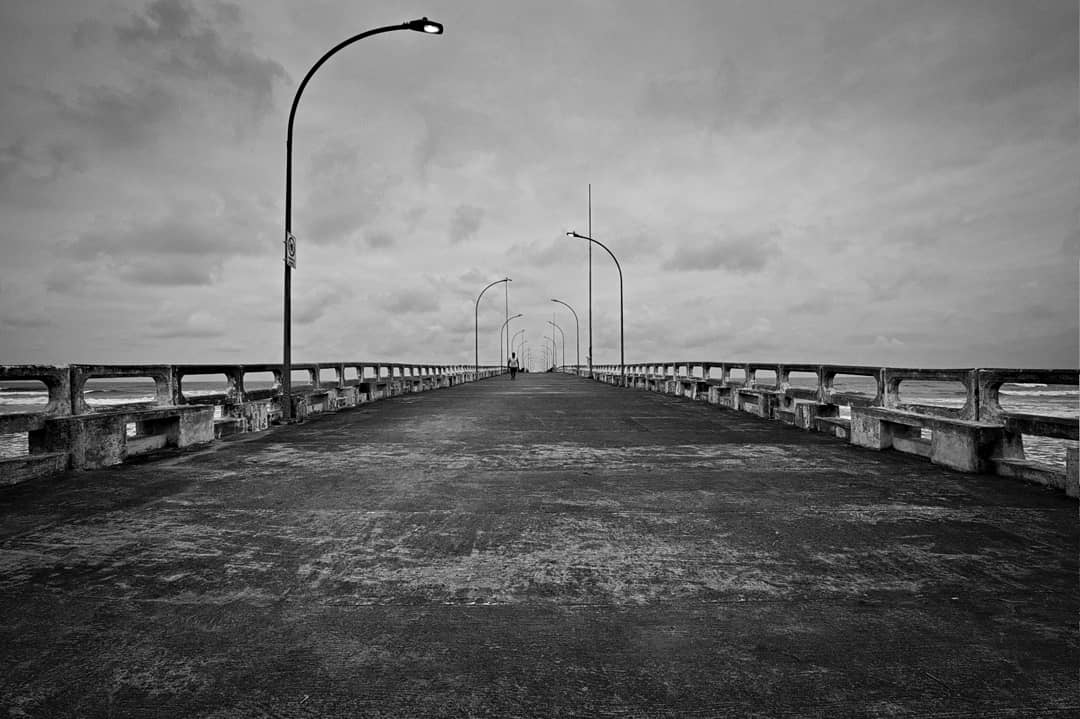
\includegraphics[scale=0.15]{plataforma.jpg}
    \caption{A plataforma de pesca.}
    \label{fig:plataforma}
\end{figure}

O argumento opcional recebe os parâmetros para escalonamento, dimensão, rotação etc. Veja os exemplos:

\begin{footnotesize}
\begin{verbatim}
\includegraphics[width=3cm, height=4cm]{logo.png}
\includegraphics[width=\textwidth]{lua.jpg}
\includegraphics[scale=1.2, angle=45]{foto.jpg}
\end{verbatim}
\end{footnotesize}

Por recomendação, a extensão do arquivo pode ser omitida, assim o \LaTeX\ irá procurar por todos os formatos suportados de imagens.

\subsection*{Posicionamento}
\addcontentsline{toc}{subsection}{Posicionamento}

O carregamento da imagem torna-se mais preciso se estiver no ambiente \texttt{\{figure\}}. Com este ambiente podemos especificar o parâmetro do posicionamento:
\begin{footnotesize}
\begin{verbatim}
\begin{figure}[h!]
    \centering
    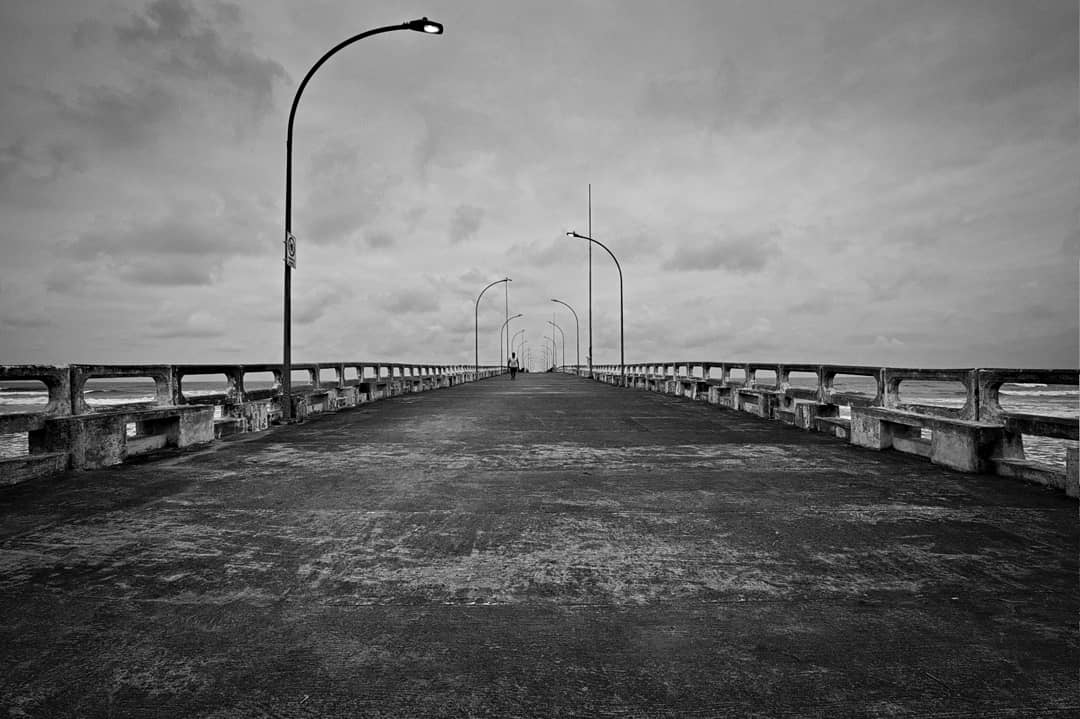
\includegraphics[scale=0.2]{plataforma.jpg}
    \caption{A plataforma de pesca.}
    \label{fig:plataforma}
\end{figure}
\end{verbatim}
\end{footnotesize}

\begin{tabular}{lp{10cm}}
\textbf{Parâmetro} & \textbf{Posição}
\\
\texttt{h \footnotesize{(here)}} & Posição flutuante aqui mesmo.
\\
\texttt{t \footnotesize{(top)}} & No topo da página.
\\
\texttt{b \footnotesize{(bottom)}} & No pé da página.
\\
\texttt{p \footnotesize{(page)}} & Coloca na página flutuante especial.
\\
\texttt{!\ \footnotesize{(override)}} & Sobrepõe o cálculo do \LaTeX\ para a posição flutuante.
\\
\end{tabular}

\newpage
Adicionando o pacote \texttt{\{wrapfig\}}, o texto ganha a possibilidade de envolver a imagem carregada. Para isso usa-se o ambiente \texttt{\{wrapfig\}}. Segue uma ilustração:

\begin{wrapfigure}{r}{0.35\textwidth}
	\centering
	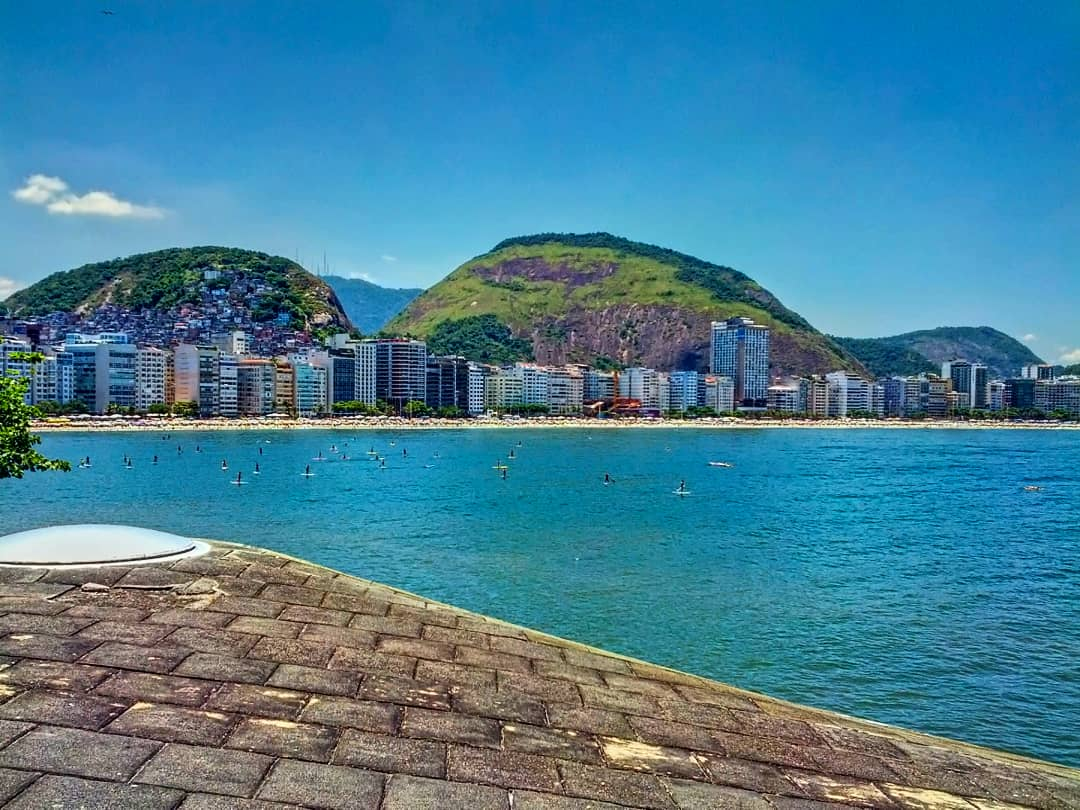
\includegraphics[width=0.35\textwidth]{copacabana.jpg}
\end{wrapfigure}

\lipsum[1-2]

\chapter*{Conclusão}
\addcontentsline{toc}{chapter}{Conclusão}

\section*{Considerações}
\addcontentsline{toc}{section}{Considerações}

O \LaTeX\ possui zilhões de comandos e quase sempre há mais de uma solução possível para formatar um conteúdo. Entretanto, o \LaTeX padrão não possui todos os comandos instalados, trazendo apenas o básico, sendo assim, existe a necessidade desta adição de pacotes. Os pacotes implementam novos comandos ao \LaTeX.

Coloquei alguns pacotes neste arquivo e nem todos estão sendo usados nos comandos. Estão aqui somente para você saber que eles existem, pois são relativamente famosos.

É muito comum ter pacotes que são aprimoramentos ou reescrita de outros. Alguns pacotes pedem até uma certa ordem no carregamento. O manual de cada um deles esclarece estes detalhes. Consulte o manual de cada pacote para conhecer mais possibilidades de formatação.

\section*{Onde saber mais} \label{sec:outrossites}
\addcontentsline{toc}{section}{Onde saber mais}

\begin{itemize}
	\setlength\itemsep{0em}
	\item \href{http://www.tex.uniyar.ac.ru/doc/latex2e.pdf}{\LaTeXe\ The macro package for \TeX}
	\item \href{https://www.ctan.org}{Comprehensive TeX Archive Network (CTAN)}
	\item \href{http://www.tug.org/}{TeX Users Group (TUG)}
	\item \href{https://tobi.oetiker.ch/lshort/lshort.pdf}{The Not So Short Introduction to \LaTeXe}
	\item \href{http://latex.silmaril.ie/formattinginformation/index.html}{Formatting Information - An introduction to typesetting with \LaTeX}
	\item \href{https://latexref.xyz/dev/latex2e.pdf}{\LaTeXe: An unofficial reference manual}
	\item \href{https://www.maths.tcd.ie/~dwilkins/LaTeXPrimer/GSWLaTeX.pdf}{Getting Started with \LaTeX}
	\item \href{http://linorg.usp.br/CTAN/info/lshort/portuguese/pt-lshort.pdf}{Uma não tão pequena introdução ao \LaTeXe}
	\item \href{https://en.wikibooks.org/wiki/LaTeX}{Wikibooks \LaTeX}
	\item \href{http://linorg.usp.br/CTAN/info/symbols/comprehensive/symbols-a4.pdf}{The Comprehensive \LaTeX\ Symbol List}
\end{itemize}




\begin{comment}

\begin{center}
\scalebox{0.60} {
\begin{tikzpicture}
\genealogytree[template=signpost] {
	parent{
		g[neuter]{\huge{filha}}
		c[neuter]{\huge{filha}}
		c[neuter]{\huge{filho}}
		parent{
			g[neuter]{\huge{pai}}
			p[neuter]{\huge{avô}}
			p[neuter]{\huge{avó}}
		}
		p[neuter]{\huge{mãe}}
	}
}
\end{tikzpicture}
}
\end{center}


\tikzstyle{retangulo} = [rectangle, minimum width=3cm, minimum height=2.2cm, text centered, text width=3cm, draw=black, fill=lightgray!30, rounded corners]
\tikzstyle{traco} = [thick,-]

\begin{center}
\scalebox{0.50} {
\begin{tikzpicture} [node distance=2.5cm]
\node (membro1) [retangulo] {
	\textcolor{teal!70!black}{\large{\textbf{Avó A}}} \par \textcolor{purple!70!black}{\large{\textbf{Esposa D}}} \par \textcolor{olive!70!black}{\large{\textbf{Mãe E}}}};
\node (membro2) [retangulo, below of=membro1] {
	\textcolor{purple!70!black}{\large{\textbf{Marido C}}} \par \textcolor{blue!70!black}{\large{\textbf{Pai I}}} \par \textcolor{olive!70!black}{\large{\textbf{Filho E}}} \par \textcolor{violet!70!black}{\large{\textbf{Irmão G}}}};
\node (membro3) [retangulo, right of=membro2, xshift=4cm] {
	\textcolor{teal!70!black}{\large{\textbf{Avó B}}} \par \textcolor{purple!70!black}{\large{\textbf{Esposa C}}} \par \textcolor{olive!70!black}{\large{\textbf{Mãe F}}}};
\node (membro4) [retangulo, below of=membro2, xshift=3.5cm] {
	\textcolor{teal!70!black}{\large{\textbf{Neta A}}} \par \textcolor{blue!70!black}{\large{\textbf{Filha I}}} \par
	\textcolor{black!80}{\large{\textbf{Solteira}}} \par
	\textcolor{violet!70!black}{\large{\textbf{Irmã H}}}};
\node (membro5) [retangulo, below of=membro3, yshift=-2.5cm] {
	\textcolor{purple!70!black}{\large{\textbf{Marido D}}} \par \textcolor{blue!70!black}{\large{\textbf{Pai J}}} \par \textcolor{olive!70!black}{\large{\textbf{Filho F}}} \par \textcolor{violet!70!black}{\large{\textbf{Irmão H}}}};
\node (membro6) [retangulo, below of=membro5, xshift=-5cm] {
	\textcolor{teal!70!black}{\large{\textbf{Neta B}}} \par \textcolor{blue!70!black}{\large{\textbf{Filha J}}} \par
	\textcolor{black!80}{\large{\textbf{Solteira}}} \par
	\textcolor{violet!70!black}{\large{\textbf{Irmã G}}}};

\draw [traco] (membro1) -- (membro2);
\draw [traco] (membro2) -- (membro3);
\draw [traco] (membro2) -| (membro4);
\draw [traco] (membro3) -- (membro5);
\draw [traco] (membro1) -- (-2,0) |- (membro5);
\draw [traco] (membro5) -| (membro6);
\end{tikzpicture}
}
\end{center}

\end{comment}

\chapter*{Colofão}
\addcontentsline{toc}{chapter}{Colofão}

Este eBook foi desenvolvido usando o sistema de preparação de documento \LaTeXe\ e editado com o software TeXstudio no sistema operacional Linux Fedora. O documento foi convertido para o formato PDF pelo TeX Live com o pdfTeX. O corpo do texto utiliza a fonte Computer Modern, no tamanho 12pt e as páginas possuem o tamanho A4, com três centímetros nas margens superior e esquerda, e com 2,5 centímetros nas margens direita e inferior.

As imagens da capa e da contracapa foram obtidas pelo website Pexels.com. A fotografia da capa foi obtida no endereço https:// www.pexels.com/ photo/ photo-of-clouds-during-daytime-2088205/ e a fotografia da contracapa foi obtida no endereço https:// www.pexels.com/ photo/ photo-of-airplane-with-smoke-trail-2088203/. Ambas estão creditadas a Eberhard Grossgasteiger.

O código-fonte deste Tutorial foi compilado em \today.\par

\backmatter

\nopagecolor

\begin{center}
	\AddToShipoutPictureBG*{
\includegraphics[width=\paperwidth,height=\paperheight]{airplane.jpg}}
	\thispagestyle{empty}
	\renewcommand{\thepage}{fim}
\end{center}

\end{document}
